\hypertarget{nodemcu}{%
\section{NodeMCU}\label{nodemcu}}

\begin{frame}{NodeMCU hardware}
\protect\hypertarget{nodemcu-hardware}{}

\includegraphics{images/NodeMCU-–-Board-de-desarrollo-con-módulo-ESP8266-WiFi-y-Lua-4.jpg}

\end{frame}

\begin{frame}{NodeMCU hardware}
\protect\hypertarget{nodemcu-hardware-1}{}

\begin{center}
\begin{tikzpicture}

\path
    (0, 0) node(flash)[draw, rectangle,
    minimum height=1cm, minimum width=2cm] {Flash}

    (0, 1.5) node(esp8266)[draw, rectangle,
    minimum height=1cm, minimum width=2cm] {ESP8266}

    (3.5, 1.5) node(cp201x)[draw, rectangle,
    minimum height=0.75cm, minimum width=1cm]
    {CP201x}

    (5.5, 1.5) node(usb)[]
    {USB}
;

\draw[-] (esp8266) -- node[node font=\footnotesize, right]{QSPI} (flash);
\draw[-] (esp8266) -- node[node font=\footnotesize, above]{UART} (cp201x) -- (usb);

\node[rectangle, draw, fit=(esp8266) (flash), inner sep=2 mm,
    label={[name=esp12_label,anchor=south]ESP-12}]
    (esp12){};

\node[rectangle, draw, thick, fit=(esp12_label) (esp12) (cp201x), inner sep=3 mm,
    label={[anchor=north]south:NodeMCU}]
    (nodemcu){};

\end{tikzpicture}

\end{center}

\end{frame}

\begin{frame}{ESP8266 software layers}
\protect\hypertarget{esp8266-software-layers}{}

\begin{center}
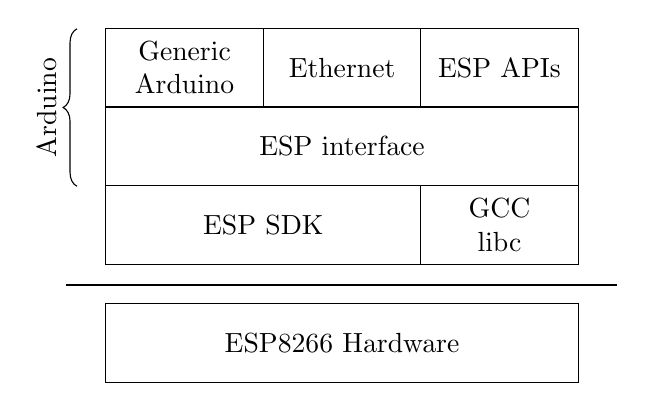
\begin{tikzpicture}

\node (rect_hw) [rectangle, draw, anchor=south west,
    minimum width=6 cm, minimum height=1 cm,
    label={[anchor=south]center:ESP8266 Hardware}] at (0, 0) {};

\draw[thick] (-0.5, 1.25) -- (6.5, 1.25) ;

\node  [rectangle, draw, anchor=south west,
    minimum width=4 cm, minimum height=1 cm,
    label={[anchor=south]center:ESP SDK}] at (0, 1.5) {};

\node [rectangle, draw, anchor=south west,
    minimum width=2 cm, minimum height=1 cm,
    label={[align=center, text width=1cm]center:GCC  libc}] at (4, 1.5) {};

\node [rectangle, draw, anchor=south west,
    minimum width=6 cm, minimum height=1 cm,
    label={[anchor=south]center:ESP interface}] at (0, 2.5) {};

\node [rectangle, draw, anchor=south west,
    minimum width=2 cm, minimum height=1 cm,
    label={[align=center, text width= 2cm]center:Generic Arduino}] at (0, 3.5) {};

\node [rectangle, draw, anchor=south west,
    minimum width=2 cm, minimum height=1 cm,
    label={[align=center, text width= 2cm]center:Ethernet}] at (2, 3.5) {};

\node [rectangle, draw, anchor=south west,
    minimum width=2 cm, minimum height=1 cm,
    label={[align=center, text width= 2cm]center:ESP APIs}] at (4, 3.5) {};

\draw [decorate, decoration={brace,amplitude=5pt, raise=-4pt}] (-0.5,2.5) -- (-0.5,4.5) node [black,midway,rotate=90, above] {Arduino};


\end{tikzpicture}

\end{center}

\end{frame}

\begin{frame}{ESP8266 + Arduino}
\protect\hypertarget{esp8266-arduino}{}

\begin{itemize}
\tightlist
\item
  Standard Arduino IDE
\item
  ESP8266 Arduino core

  \begin{itemize}
  \tightlist
  \item
    https://github.com/esp8266/Arduino
  \end{itemize}
\end{itemize}

\end{frame}

\begin{frame}{Arduino IDE}
\protect\hypertarget{arduino-ide}{}

\includegraphics{images/arduino-ide.png}

\end{frame}

\begin{frame}[fragile]{Arduino code structure}
\protect\hypertarget{arduino-code-structure}{}

\begin{Shaded}
\begin{Highlighting}[]
\DataTypeTok{void}\NormalTok{ setup() \{}
    \CommentTok{// Called once}
\NormalTok{\}}

\DataTypeTok{void}\NormalTok{ loop() \{}
    \CommentTok{// Called repeatedly}
\NormalTok{\}}
\end{Highlighting}
\end{Shaded}

\note{MCU programming is often structured into:

\begin{itemize}
\tightlist
\item
  Configure

  \begin{itemize}
  \tightlist
  \item
    CPU
  \item
    GPIO ports
  \item
    MCU’s peripherals
  \item
    The rest of the board
  \item
    Configure application and callbacks.
  \end{itemize}
\item
  Sleep
\end{itemize}

Arduino chooses to run the cpu at 100\% instead of the sleep step..}

\end{frame}

\begin{frame}[fragile]{Arduino file structure}
\protect\hypertarget{arduino-file-structure}{}

\begin{verbatim}
foo/
  foo.ino
  config.h
\end{verbatim}

\note{\texttt{foo.ino} must always be in a \texttt{foo} directory.

config.h is created by “new tab”.}

\end{frame}

\begin{frame}[fragile]{Generic Arduino APIs}
\protect\hypertarget{generic-arduino-apis}{}

\begin{Shaded}
\begin{Highlighting}[]
\CommentTok{// Pin: D0, D1, etc.}
\CommentTok{// Mode: OUTPUT, INPUT, INPUT_PULLUP}
\DataTypeTok{void}\NormalTok{ pinMode(}\DataTypeTok{uint8_t}\NormalTok{ pin, }\DataTypeTok{uint8_t}\NormalTok{ mode);}

\CommentTok{// State: HIGH, LOW, true/false, 1/0}
\DataTypeTok{void}\NormalTok{ digitalWrite(}\DataTypeTok{uint8_t}\NormalTok{ pin, }\DataTypeTok{uint8_t}\NormalTok{ state);}
\DataTypeTok{int}\NormalTok{ digitalRead(}\DataTypeTok{uint8_t}\NormalTok{ pin);}

\DataTypeTok{unsigned} \DataTypeTok{long}\NormalTok{ now millis();}
\DataTypeTok{unsigned} \DataTypeTok{long}\NormalTok{ now micros();}
\end{Highlighting}
\end{Shaded}

\end{frame}

\begin{frame}[fragile]{ESP Arduino APIs}
\protect\hypertarget{esp-arduino-apis}{}

\begin{Shaded}
\begin{Highlighting}[]
\KeywordTok{class}\NormalTok{ \{}
    \DataTypeTok{void}\NormalTok{ restart();}
    \DataTypeTok{uint32_t}\NormalTok{ getFreeHeap();}
    \DataTypeTok{uint32_t}\NormalTok{ getChipId();}

\NormalTok{    ...}
\NormalTok{\} ESP;}

\CommentTok{// Usage}
\NormalTok{ESP.restart();}
\end{Highlighting}
\end{Shaded}

\end{frame}

\begin{frame}[fragile]{ESP Arduino APIs}
\protect\hypertarget{esp-arduino-apis-1}{}

\begin{Shaded}
\begin{Highlighting}[]
\KeywordTok{class}\NormalTok{ \{}
\NormalTok{    String macAddress();}

    \DataTypeTok{wl_status_t}\NormalTok{ status();}
    \DataTypeTok{int32_t}\NormalTok{ RSSI();}

\NormalTok{    IPAddress localIP();}
\NormalTok{    IPAddress subnetMask();}
\NormalTok{    IPAddress gatewayIP();}
\NormalTok{    IPAddress dnsIP(}\DataTypeTok{uint8_t}\NormalTok{ dns_no = }\DecValTok{0}\NormalTok{);}

\NormalTok{    ...}
\NormalTok{\} WiFi;}

\CommentTok{// Usage:}

\NormalTok{Serial.println(WiFi.localIP().toString());}
\end{Highlighting}
\end{Shaded}

\note{http://arduino-esp8266.readthedocs.io/en/latest/libraries.html}

\end{frame}

\hypertarget{what-is-iot}{%
\section{What is IoT}\label{what-is-iot}}

\begin{frame}{What is IoT}
\protect\hypertarget{what-is-iot-1}{}

\begin{itemize}
\tightlist
\item
  Not “a computer connected to the internet”

  \begin{itemize}
  \tightlist
  \item
    Then it is really just another computer connected to the internet
  \end{itemize}
\item
  Must be something else

  \begin{itemize}
  \tightlist
  \item
    It is simply devices that are resource constrained

    \begin{itemize}
    \tightlist
    \item
      Usually in more than one way
    \end{itemize}
  \end{itemize}
\item
  Autonomous operation, the connection might not be permanent
\end{itemize}

\end{frame}

\begin{frame}{IoT is just a concept}
\protect\hypertarget{iot-is-just-a-concept}{}

\begin{itemize}
\tightlist
\item
  \emph{The Internet of Things (IoT) is the network of physical devices,
  vehicles, home appliances and other items embedded with electronics,
  software, sensors, actuators, and connectivity which enables these
  objects to connect and exchange data.}\footnote<.->{Wikipedia
    “Internet of Things”}
\end{itemize}

\end{frame}

\begin{frame}{What is an IoT Device?}
\protect\hypertarget{what-is-an-iot-device}{}

\note{As for their definition.

What differentiates a computer from an IoT device?}

\end{frame}

\begin{frame}{What is an IoT Device?}
\protect\hypertarget{what-is-an-iot-device-1}{}

\begin{itemize}
\tightlist
\item
  Constrained in (one or more of):

  \begin{itemize}
  \tightlist
  \item
    Memory
  \item
    CPU
  \item
    Network bandwidth and/or latency
  \item
    Storage
  \end{itemize}
\item
  Has connectivity

  \begin{itemize}
  \tightlist
  \item
    Bluetooth
  \item
    Wi-Fi
  \item
    NB-IoT
  \item
    LTE Cat-M
  \item
    LoRA
  \item
    Proprietary radio
  \end{itemize}
\end{itemize}

\note{Might not have:

\begin{itemize}
\tightlist
\item
  RTC
\end{itemize}

Extra features:

\begin{itemize}
\tightlist
\item
  IR
\item
  UART
\item
  CAN
\end{itemize}

Sparkfun and Adafruit etc sell modules with all of these technologies.}

\end{frame}

\begin{frame}{IoT Devices - Bluetooth 4/5 chips}
\protect\hypertarget{iot-devices---bluetooth-45-chips}{}

\begin{longtable}[]{@{}llllll@{}}
\toprule
Chip & CPU & Freq & RAM & Flash & Price\tabularnewline
\midrule
\endhead
nRF52810 & Cortex-M4 & 64 MHz & 24k & 192k & \$1.88\tabularnewline
nRF52832 & Cortex-M4F & & 32k & 256k & \$2.54\tabularnewline
& & & 64k & 512k & \$2.59\tabularnewline
nRF52840 & Cortex-M4F & & 256k & 1024k & \$3.85\tabularnewline
\bottomrule
\end{longtable}

\begin{itemize}
\tightlist
\item
  nRF52810: High performance, entry-level Bluetooth 4/ANT/2.4GHz SoC
\item
  nRF52832: High performance Bluetooth 4/ANT/2.4GHz SoC
\item
  nRF52840: Advanced multi-protocol System-on-Chip Supporting: Bluetooth
  5, ANT/ANT+, 802.15.4 and 2.4GHz proprietary
\end{itemize}

\note{All quantities are 1000 pieces

nRF51:
https://www.digikey.no/products/en/rf-if-and-rfid/rf-transceiver-ics/879?k=nrf51822

nRF52832: these have different packagings, not only difference price

https://www.digikey.no/products/en/rf-if-and-rfid/rf-transceiver-ics/879?FV=1c0001\%2Cffe0036f\&quantity=3000\&ColumnSort=1000011\&page=1\&k=nrf52832\&pageSize=500\&pkeyword=nrf52810

nRF52810: High performance, entry-level Bluetooth 4/ANT/2.4GHz SoC
nRF52832: High performance Bluetooth 4/ANT/2.4GHz SoC nRF52840: Advanced
multi-protocol System-on-Chip Supporting: Bluetooth 5, ANT/ANT+,
802.15.4 and 2.4GHz proprietary}

\end{frame}

\begin{frame}{IoT Devices - LoRA}
\protect\hypertarget{iot-devices---lora}{}

\begin{block}{Modules}

\begin{longtable}[]{@{}lll@{}}
\toprule
Module & Data Rate & Price\tabularnewline
\midrule
\endhead
RN2483A-I/RM104 & & \$12.05 @ 250\tabularnewline
CMWX1ZZABZ-078 & SX1276 & \$10.74 @ 1000\tabularnewline
RF-LORA-868-SO & SX1272 & \$16.55 @ 1000\tabularnewline
\bottomrule
\end{longtable}

\end{block}

\begin{block}{Chips}

\begin{longtable}[]{@{}ll@{}}
\toprule
Chip & Price\tabularnewline
\midrule
\endhead
SX1281 & \$3.23\tabularnewline
SX1272 & \$4.25\tabularnewline
SX1276 & \$4.25\tabularnewline
SX1279 & \$4.74\tabularnewline
\bottomrule
\end{longtable}

\note{These modules require an external MCU, so does the chips.}

\end{block}

\end{frame}

\begin{frame}{IoT Devices - NB-IoT}
\protect\hypertarget{iot-devices---nb-iot}{}

\begin{longtable}[]{@{}ll@{}}
\toprule
Module & Price\tabularnewline
\midrule
\endhead
uBlox SARA-N210 & \textasciitilde{}\$10 @ 100\tabularnewline
Sierra Wireless HL7800\_1103933 & \$15.72\tabularnewline
\bottomrule
\end{longtable}

\end{frame}

\begin{frame}{IoT Devices - Wi-Fi}
\protect\hypertarget{iot-devices---wi-fi}{}

\begin{longtable}[]{@{}llllll@{}}
\toprule
Chip & CPU & Freq & ROM & RAM & Price\tabularnewline
\midrule
\endhead
ESP8266 & Tensilica L106 & 160 MHz & N/A & \textasciitilde{}50 kB &
\textless{} \$1\tabularnewline
\bottomrule
\end{longtable}

ESP32 - dual cpu, Wi-Fi, Bluetooth 4 ESP32-D0WDQ6 2x Xtensa @ 160MHz \$
4.53 @ 10

\note{The ESP8266’s RAM depends on which firmware stack is used.
Physical is probably 128k or most likely 64k.}

\end{frame}

\begin{frame}{ESP8266 details - Power usage}
\protect\hypertarget{esp8266-details---power-usage}{}

\begin{longtable}[]{@{}lr@{}}
\toprule
\begin{minipage}[b]{0.35\columnwidth}\raggedright
State\strut
\end{minipage} & \begin{minipage}[b]{0.22\columnwidth}\raggedleft
Current usage\strut
\end{minipage}\tabularnewline
\midrule
\endhead
\begin{minipage}[t]{0.35\columnwidth}\raggedright
Off\strut
\end{minipage} & \begin{minipage}[t]{0.22\columnwidth}\raggedleft
0.5 µA\strut
\end{minipage}\tabularnewline
\begin{minipage}[t]{0.35\columnwidth}\raggedright
Deep sleep with RTC\strut
\end{minipage} & \begin{minipage}[t]{0.22\columnwidth}\raggedleft
20 µA\strut
\end{minipage}\tabularnewline
\begin{minipage}[t]{0.35\columnwidth}\raggedright
Light sleep (with Wi-Fi)\strut
\end{minipage} & \begin{minipage}[t]{0.22\columnwidth}\raggedleft
1 mA\strut
\end{minipage}\tabularnewline
\begin{minipage}[t]{0.35\columnwidth}\raggedright
Sleep with peripherials\strut
\end{minipage} & \begin{minipage}[t]{0.22\columnwidth}\raggedleft
15 mA\strut
\end{minipage}\tabularnewline
\begin{minipage}[t]{0.35\columnwidth}\raggedright
TX\strut
\end{minipage} & \begin{minipage}[t]{0.22\columnwidth}\raggedleft
170 mA\strut
\end{minipage}\tabularnewline
\bottomrule
\end{longtable}

\note{Datasheet page 18}

\end{frame}

\hypertarget{going-back-to-basics}{%
\section{Going back to basics}\label{going-back-to-basics}}

\begin{frame}{What is the internet again?}
\protect\hypertarget{what-is-the-internet-again}{}

\end{frame}

\begin{frame}{TCP/IP Layers}
\protect\hypertarget{tcpip-layers}{}

\begin{center}
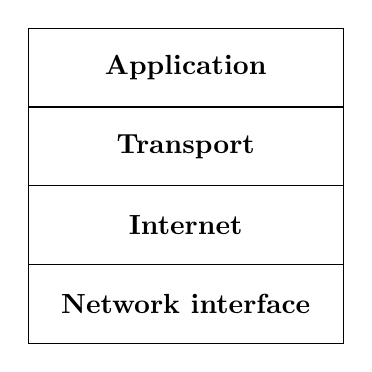
\begin{tikzpicture}[
mybox/.style={draw, rectangle, minimum width=4cm, minimum height=1 cm,font=\bfseries}
]

%\draw (0,0) rectangle (3cm, 1cm) {wat};

\node at (0, -0) [mybox] {Application};
\node at (0, -1) [mybox] {Transport};
\node at (0, -2) [mybox] {Internet};
\node at (0, -3)[mybox] {Network interface};

\end{tikzpicture}

\end{center}

\end{frame}

\begin{frame}{Packet encapsulation}
\protect\hypertarget{packet-encapsulation}{}

\begin{center}
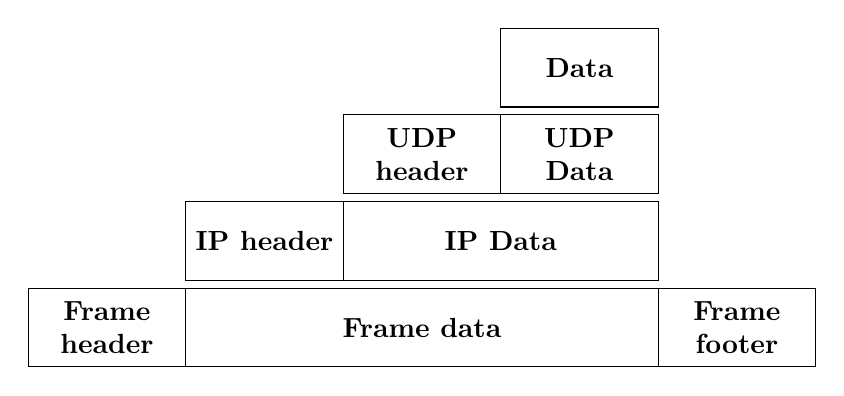
\begin{tikzpicture}[
mybox/.style={
    draw,
    rectangle,
    minimum height=1 cm,
    anchor=west,
    align=center,
    font=\bfseries}
]

%\draw (0,0) rectangle (3cm, 1cm) {wat};

\node at (0 cm, 0 cm) [mybox, minimum width=2cm, text width=1.7cm] {Frame header};
\node at (2 cm, 0 cm) [mybox, minimum width=6cm] {Frame data};
\node at (8 cm, 0 cm) [mybox, minimum width=2cm, text width=1.7cm] {Frame footer};

\node at (2 cm, 1.1 cm) [mybox, minimum width=2cm] {IP header};
\node at (4 cm, 1.1 cm) [mybox, minimum width=4cm] {IP Data};

\node at (4 cm, 2.2 cm) [mybox, minimum width=2cm, text width=1.7 cm] {UDP header};
\node at (6 cm, 2.2 cm) [mybox, minimum width=2cm, text width=1.7 cm] {UDP Data};

\node at (6 cm, 3.3 cm) [mybox, minimum width=2cm, text width=1.7 cm] {Data};

\end{tikzpicture}

\end{center}

\end{frame}

\begin{frame}{Network interface}
\protect\hypertarget{network-interface}{}

\begin{itemize}
\tightlist
\item
  Ethernet

  \begin{itemize}
  \tightlist
  \item
    10BASE5, 10BASE2, 10BASE-T / 100BASE-TX / 1000BASE-TX
  \end{itemize}
\item
  Wi-Fi

  \begin{itemize}
  \tightlist
  \item
    802.11a/b/g/n
  \end{itemize}
\item
  RS-232
\end{itemize}

\note{Ethernet: Hubs and switches (that act on this level) is not on
it’s own layer. It is more of a implementation detail in the
architecture diagram.

RS-232 signaling is used in \emph{all} MCUs, many have several ports
available. It is extremely flexible, both used for implementing
applications and debugging. Frequently an easy way to hack embedded
devices. “USB dongles”, “USB TTL” all use RS-232 signaling.

Note that this only applies to its logical signals, not voltage levels.
The signaling does not specify any max data rate, very high rates
(\textgreater{}= 1Mbps) is often supported.}

\end{frame}

\begin{frame}{Internet}
\protect\hypertarget{internet}{}

\begin{itemize}
\tightlist
\item
  IP
\item
  ICMP
\end{itemize}

\end{frame}

\begin{frame}{Transport}
\protect\hypertarget{transport}{}

\begin{itemize}
\tightlist
\item
  TCP
\item
  UDP
\item
  SCTP
\item
  QUIC
\end{itemize}

\end{frame}

\begin{frame}{Layer 7: Application Layer}
\protect\hypertarget{layer-7-application-layer}{}

\begin{itemize}
\tightlist
\item
  HTTP
\item
  DNS
\item
  MQTT
\item
  CoAP
\item
  (everything else..)
\end{itemize}

\end{frame}

\begin{frame}{Details: IP}
\protect\hypertarget{details-ip}{}

\begin{center}
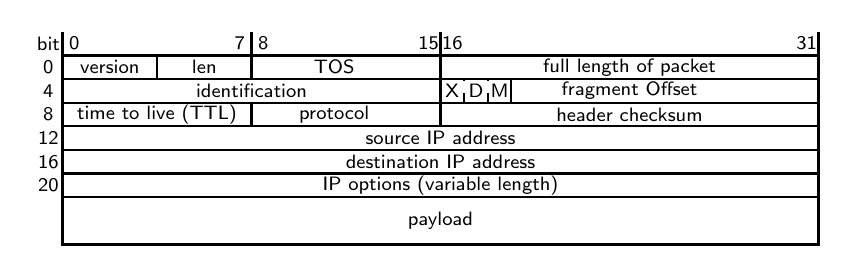
\begin{tikzpicture}[scale=0.30]
    \sffamily
    \foreach \x in {0,7,8,15,16,31} % {0,...,32}
        \node at (\x+0.5,20.5) {\scriptsize \x};
%   \foreach \x in {0,...,31}
%       \node at (\x+0.5,13.5) {\scriptsize \x};
    \foreach \x in {0,8,16,32} % {0,...,32}
        \draw[thick] (\x,20) -- (\x,21);
    \foreach \x in {0,...,32}
        \draw[thick] (\x,14) -- (\x,20);
%   \foreach \x in {0,...,32}
%       \draw[thick] (\x,13) -- (\x,14);
    \node[thick] (bit1) at (-0.6,20.5) {\scriptsize bit};
%   \node[thick] (bit2) at (-0.6,13.5) {\scriptsize bit};
        
\iffalse
    \draw [<->, thick] (-0.6, 19.9) -- (-0.6,15.1);
    \draw [thick] (-1, 20) -- (-0.1,20);
    \draw [thick] (-1, 15) -- (-0.1,15);
    \node[fill=white] at (-1.1,17.5) {\tiny 20 bytes};
\fi
    \foreach \y/\v in {0,4,8,12,16,20}
        \node at (-0.6,{19.5-(\v / 4)}) {\scriptsize \v};

    \filldraw[thick,draw=black, fill=white] (0,20) rectangle (4,19); \node (mode) at (2,19.5) {\scriptsize version};
    \filldraw[thick,draw=black, fill=white] (4,20) rectangle (8,19); \node (mode) at (6,19.5) {\scriptsize len};
%   \draw[thick, draw=black, fill=white] (8,20) rectangle (16,19); \node (stratum) at (11.5,19.5) {\scriptsize type of service (TOS)};
    \draw[thick, draw=black, fill=white] (8,20) rectangle (16,19); \node (stratum) at (11.5,19.5) {\scriptsize TOS};
    \draw[thick, draw=black, fill=white] (16,20) rectangle (32,19); \node (li) at (24,19.5) {\scriptsize full length of packet};
    \filldraw[thick,draw=black, fill=white] (0,19) rectangle (16,18); \node (mode) at (8,18.5) {\scriptsize identification};
%   \draw[thick, draw=black] (16,19) rectangle (19,18); \filldraw[white] (16.5,18.43) rectangle (19,18.88); \node [](li) at (17.5,18.67) {\tiny IP flags}; \node at (16.5,18.25) {\tiny x};\node at (17.5,18.25) {\tiny D};\node at (18.5,18.25) {\tiny M};
    \draw[thick, draw=black] (16,19) rectangle (19,18); \filldraw[white] (16.5,18.43) rectangle (19,18.88); \node at (16.5,18.5) {\scriptsize X};\node at (17.5,18.5) {\scriptsize D};\node at (18.5,18.5) {\scriptsize M};
    \draw[thick, draw=black, fill=white] (19,19) rectangle (32,18); \node (li) at (24,18.5) {\scriptsize fragment Offset};
    \filldraw[thick,draw=black, fill=white] (0,18) rectangle (8,17); \node (mode) at (4,17.5) {\scriptsize time to live (TTL)};
    \draw[thick, draw=black, fill=white] (8,18) rectangle (16,17); \node (stratum) at (11.5,17.5) {\scriptsize protocol};
    \draw[thick, draw=black, fill=white] (16,18) rectangle (32,17); \node (li) at (24,17.5) {\scriptsize header checksum};
    \filldraw[thick,draw=black, fill=white] (0,17) rectangle (32,16); \node (mode) at (16,16.5) {\scriptsize source IP address};
    \filldraw[thick,draw=black, fill=white] (0,16) rectangle (32,15); \node (mode) at (16,15.5) {\scriptsize destination IP address};
    \draw[thick,draw=black, fill=white] (0,15) rectangle (32,14);
%   \draw[thick,draw=black, fill=white] (0,15) rectangle (31.5,14);
%   \draw[fill=white, draw=white] (31.4,15) rectangle (31.6,16);
%   \draw[thick]  (31.5,14.97)  decorate [decoration=saw] { -- (31.5,14.02)};
    \node (mode) at (16,14.5) {\scriptsize IP options (variable length)};

    \filldraw[thick,draw=black, fill=white] (0,12) rectangle (32,14); \node (mode) at (16,13) {\scriptsize payload};

\end{tikzpicture}

\end{center}

\end{frame}

\begin{frame}{Details: UDP}
\protect\hypertarget{details-udp}{}

\begin{center}
\scalebox{0.5}{

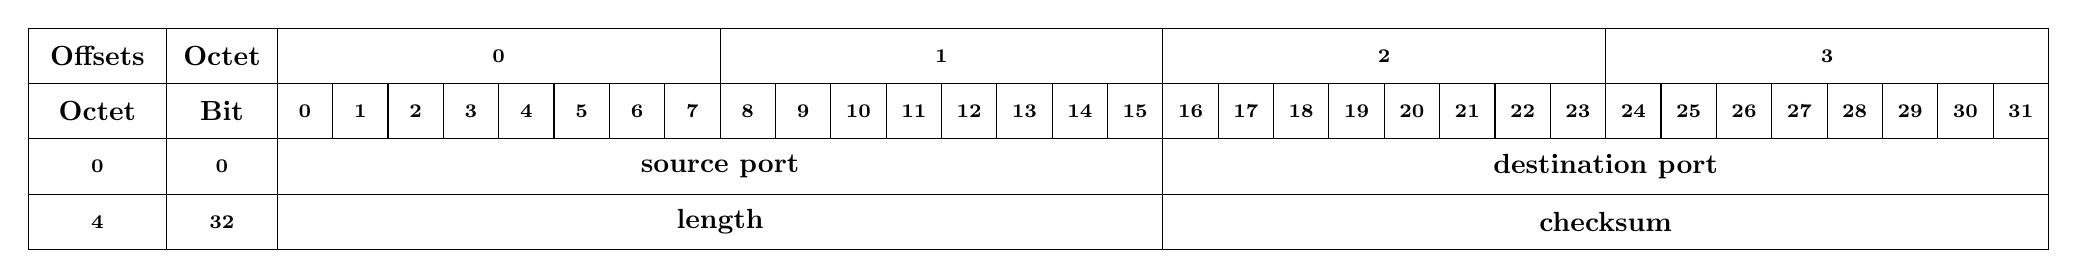
\begin{tikzpicture}[
every node/.style={font=\bfseries}
]

\path 
(-6.5em, 2em) node[draw, rectangle, minimum width=5em, minimum height=2em] {Offsets}
(-6.5em, 0em) node[draw, rectangle, minimum width=5em, minimum height=2em] {Octet}
(-2em, 2em) node[draw, rectangle, minimum width=4em, minimum height=2em] {Octet}
(-2em, 0em) node[draw, rectangle, minimum width=4em, minimum height=2em] {Bit}

(16em, -2em) node[draw, rectangle, minimum width=32em, minimum height=2em] {source port}
(48em, -2em) node[draw, rectangle, minimum width=32em, minimum height=2em] {destination port}
(16em, -4em) node[draw, rectangle, minimum width=32em, minimum height=2em] {length}
(48em, -4em) node[draw, rectangle, minimum width=32em, minimum height=2em] {checksum}
;

\foreach \x in {0,...,3}
    \node[draw, rectangle, minimum width=16em, minimum height=2em] at (\x * 16em + 8em, 2em) {\scriptsize \x};
\foreach \x in {0,...,31}
    \node[draw, rectangle, minimum width=2em, minimum height=2em] at (\x * 2em + 1em, 0em) {\scriptsize \x};

\node[draw, rectangle, minimum width=4em, minimum height=2em] at (-2em, -2em) {\scriptsize 0};
\node[draw, rectangle, minimum width=4em, minimum height=2em] at (-2em, -4em) {\scriptsize 32};

\node[draw, rectangle, minimum width=5em, minimum height=2em] at (-6.5em, -2em) {\scriptsize 0};
\node[draw, rectangle, minimum width=5em, minimum height=2em] at (-6.5em, -4em) {\scriptsize 4};

\end{tikzpicture}

}

\end{center}

\end{frame}

\hypertarget{lecture-mqtt}{%
\section{Lecture: MQTT}\label{lecture-mqtt}}

\begin{frame}{MQTT}
\protect\hypertarget{mqtt}{}

\begin{itemize}
\tightlist
\item
  \emph{Message Queuing Telemetry Transport}
\item
  \href{https://en.wikipedia.org/wiki/MQTT}{Wikipedia: MQTT}
\end{itemize}

\note{MQTT is \emph{the} standard for IoT applications (and lots of
other useful stuff to). Using HTTP is just silly.

Supports SSL, and requires TCP.

Has UDP-like semantics with “fire and forget” but on a higher level (the
message always have to be delivered and ACKed by the broker, not it’s
final recipient.

Version 3.1.1 er den som gjelder, V 3.1 er rar, de andre finnes ikke
(før standardisering).}

\end{frame}

\begin{frame}{Device and application architecture with MQTT}
\protect\hypertarget{device-and-application-architecture-with-mqtt}{}

\begin{center}
\begin{tikzpicture}

\path
    (-3 cm, 0) node (c1_label) {Device \#1}
    ( 0 cm, 0) node (c2_label) {Device \#2}
    ( 3 cm, 0) node (c3_label) {Device \#3}

    (0, -3 cm) node (broker_label) {Broker}
    (0, -6 cm) node (central_label) {Central}
;

\node (c1)[draw, circle, fit=(c1_label)] {};
\node (c2)[draw, circle, fit=(c2_label)] {};
\node (c3)[draw, circle, fit=(c3_label)] {};
\node (broker)[draw, rectangle, thick, inner ysep=5 mm, inner xsep=10 mm, fit=(broker_label)] {};
\node (central) at (central_label) [draw, circle, text width=2 cm] {};

\draw[{Latex[length=4mm, round]}-{Latex[length=4mm, round]}] (c1) to [bend right] (broker);
\draw[{Latex[length=4mm, round]}-{Latex[length=4mm, round]}] (c2) -- (broker);
\draw[{Latex[length=4mm, round]}-{Latex[length=4mm, round]}] (c3) to [bend left] (broker);
\draw[{Latex[length=4mm, round]}-{Latex[length=4mm, round]}] (central) -- (broker);

\end{tikzpicture}

\end{center}

\end{frame}

\begin{frame}{MQTT - Implementations}
\protect\hypertarget{mqtt---implementations}{}

\begin{itemize}
\tightlist
\item
  Mosquitto
\item
  Eclipse Paho
\item
  RabbitMQ
\item
  ActiveMQ
\end{itemize}

\note{RabbitMQ has a separate connector that must be installed Not sure
about ActiveMQ but it is at least a part of the project so it is
releases at the same time.}

\end{frame}

\begin{frame}{MQTT Cloud Connectors}
\protect\hypertarget{mqtt-cloud-connectors}{}

\begin{itemize}
\tightlist
\item
  Cloud

  \begin{itemize}
  \tightlist
  \item
    Amazon IoT
  \item
    Google Cloud IoT
  \item
    Microsoft Azure IoT
  \item
    CloudMQTT (at Heroku)
  \end{itemize}
\item
  DIY

  \begin{itemize}
  \tightlist
  \item
    ThingMQ
  \item
    HiveMQ
  \end{itemize}
\end{itemize}

\note{In between are:

\begin{itemize}
\tightlist
\item
  self hosted
\item
  Generic bridges
\end{itemize}}

\end{frame}

\begin{frame}{MQTT - The protocol}
\protect\hypertarget{mqtt---the-protocol}{}

Agents have one of two roles:

\begin{itemize}
\tightlist
\item
  \emph{Client}

  \begin{itemize}
  \tightlist
  \item
    Publishes \emph{messages}
  \item
    Subscribes / unsubscribes to \emph{topics}
  \end{itemize}
\item
  \emph{Broker} (aka Server)

  \begin{itemize}
  \tightlist
  \item
    Handles network connections
  \item
    Keeps subscriptions
  \item
    Manages client

    \begin{itemize}
    \tightlist
    \item
      Disconnects
    \item
      \emph{(last) will}
    \end{itemize}
  \item
    Persistence of retained messages
  \end{itemize}
\end{itemize}

\note{network connections: this includes removing closed sockets,
client’s that doesn’t respons to timeouts and duplicate clients.

http://docs.oasis-open.org/mqtt/mqtt/v3.1.1/mqtt-v3.1.1.html

Subscriptions are not permanent. The connection is (unlike HTTP)
stateful.

Some messages may be persistent, but only one per topic. You will often
end up with a “proper” mq on the backend if queuing is needed.

Push vs pull, central applications can push to clients}

\end{frame}

\begin{frame}{MQTT - The protocol - MQTT Packet}
\protect\hypertarget{mqtt---the-protocol---mqtt-packet}{}

\begin{itemize}
\tightlist
\item
  Size oriented
\item
  Flags indicate type of remaining bytes

  \begin{itemize}
  \tightlist
  \item
    Packet type
  \item
    Topic name
  \item
    Payload
  \end{itemize}
\end{itemize}

\note{Only packet type + flags (1 byte) is required, everything else is
optional.

The size field is variable length encoded, 0-127 bytes is 1 byte,
128-16383 use 2 bytes etc, up to 4 bytes for 256MB payload.}

\end{frame}

\begin{frame}[fragile]{MQTT Connect}
\protect\hypertarget{mqtt-connect}{}

\begin{itemize}
\tightlist
\item
  \texttt{CONNECT}

  \begin{itemize}
  \tightlist
  \item
    \texttt{clientId}
  \item
    \texttt{username}
  \item
    \texttt{password}
  \item
    \texttt{keepAlive}
  \end{itemize}
\end{itemize}

\begin{itemize}
\tightlist
\item
  Keep alive

  \begin{itemize}
  \tightlist
  \item
    \texttt{PINGREQ}
  \item
    \texttt{PINGRESP}
  \end{itemize}
\end{itemize}

\end{frame}

\begin{frame}[fragile]{MQTT - The protocol - MQTT Topic}
\protect\hypertarget{mqtt---the-protocol---mqtt-topic}{}

\begin{itemize}
\tightlist
\item
  Topic name: \texttt{foo/bar/baz}
\item
  Topic filter

  \begin{itemize}
  \tightlist
  \item
    \texttt{foo/bar/?}
  \item
    \texttt{foo/\#}
  \end{itemize}
\end{itemize}

\end{frame}

\begin{frame}[fragile]{MQTT - The protocol - Retained message}
\protect\hypertarget{mqtt---the-protocol---retained-message}{}

Message is kept by the server even after disconnect

\begin{itemize}
\tightlist
\item
  \texttt{CONNECT}
\item
  \texttt{PUBLISH}

  \begin{itemize}
  \tightlist
  \item
    \texttt{RETAIN}
  \item
    \texttt{\$app/\$device/temperature}
  \item
    \texttt{22.3}
  \end{itemize}
\item
  \texttt{DISCONNECT}
\end{itemize}

Later on:

\begin{itemize}
\tightlist
\item
  \texttt{SUBSCRIBE}

  \begin{itemize}
  \tightlist
  \item
    \texttt{\$app/\#/temperature}
  \end{itemize}
\item
  \texttt{PUBLISH}

  \begin{itemize}
  \tightlist
  \item
    \texttt{\$app/\$device/temperature}
  \item
    \texttt{22.3}
  \end{itemize}
\end{itemize}

\note{The last PUBLISH is an incoming message}

\end{frame}

\begin{frame}[fragile]{MQTT - The protocol - Will message}
\protect\hypertarget{mqtt---the-protocol---will-message}{}

Message sent when you disconnect

Client \#1:

\begin{enumerate}
[1.]
\tightlist
\item
  \texttt{CONNECT}

  \begin{itemize}
  \tightlist
  \item
    \texttt{WILL\ TOPIC:\ \$app/\$device/online}
  \item
    \texttt{WILL\ PAYLOAD:\ 0}
  \end{itemize}
\item
  \texttt{PUBLISH}

  \begin{itemize}
  \tightlist
  \item
    \texttt{\$app/\$device/online}
  \item
    \texttt{1}
  \end{itemize}
\item
  \texttt{DISCONNECT}
\end{enumerate}

Broker

\begin{enumerate}
[1.]
\tightlist
\item
  \emph{To all subscribers} \texttt{PUBLISH}

  \begin{itemize}
  \tightlist
  \item
    \texttt{\$app/\$device/online}
  \item
    \texttt{0}
  \end{itemize}
\end{enumerate}

\end{frame}

\begin{frame}[fragile]{MQTT Topic}
\protect\hypertarget{mqtt-topic}{}

The temperature sensor:

\begin{itemize}
\tightlist
\item
  Publishes on:

  \begin{itemize}
  \tightlist
  \item
    \texttt{myapp/\$device-id/temperature}
  \item
    \texttt{myapp/\$device-id/humidity}
  \item
    \texttt{myapp/\$device-id/altert}
  \end{itemize}
\item
  Subscribes to:

  \begin{itemize}
  \tightlist
  \item
    \texttt{myapp/\$device-id/command}
  \end{itemize}
\end{itemize}

The central application:

\begin{itemize}
\tightlist
\item
  Subscribes to:

  \begin{itemize}
  \tightlist
  \item
    \texttt{myapp/\#/temperature}
  \item
    \texttt{myapp/\#/humidity}
  \end{itemize}
\item
  Publishes on:

  \begin{itemize}
  \tightlist
  \item
    \texttt{myapp/\$device-id/command}
  \end{itemize}
\end{itemize}

\note{Typical first round of implementation.

Commands can be: * load new firmware (maybe an URL and firmware
signature). * Set new calibration values * Change reading interval,
altert levels (autonomous operation)}

\end{frame}

\begin{frame}[fragile]{MQTT on Arduino}
\protect\hypertarget{mqtt-on-arduino}{}

PubSubClient is our MQTT client implementation.

\begin{Shaded}
\begin{Highlighting}[]
\NormalTok{WiFiClient wifiClient;}
\NormalTok{PubSubClient mqtt(wifiClient);}

\DataTypeTok{void}\NormalTok{ callback(}\DataTypeTok{char}\NormalTok{* topic,}
\NormalTok{              byte* payload,}
              \DataTypeTok{unsigned} \DataTypeTok{int}\NormalTok{ length);}

\DataTypeTok{void}\NormalTok{ setup() \{}
    \CommentTok{// Configure WiFi}
\NormalTok{    mqtt.setServer(mqtt_server, }\DecValTok{1883}\NormalTok{);}
\NormalTok{    mqtt.setCallback(callback);}
\NormalTok{\}}
\end{Highlighting}
\end{Shaded}

\end{frame}

\begin{frame}[fragile]{MQTT on Arduino}
\protect\hypertarget{mqtt-on-arduino-1}{}

\begin{Shaded}
\begin{Highlighting}[]
\DataTypeTok{void}\NormalTok{ loop() \{}
    \ControlFlowTok{if}\NormalTok{ (!mqtt.connected())}
\NormalTok{        reconnect();}
    \ControlFlowTok{else}
\NormalTok{        mqtt.loop();}
    \CommentTok{// Do work}
\NormalTok{\}}

\DataTypeTok{void}\NormalTok{ reconnect() \{}
    \ControlFlowTok{while}\NormalTok{ (!mqtt.}\FunctionTok{connect}\NormalTok{(client_id));}

\NormalTok{    mqtt.subscribe(topic_pattern);}
\NormalTok{\}}
\end{Highlighting}
\end{Shaded}

\note{This is blocking!}

\end{frame}

\begin{frame}[fragile]{Assignment}
\protect\hypertarget{assignment}{}

\begin{itemize}
\tightlist
\item
  \texttt{mqtt}
\end{itemize}

\end{frame}

\begin{frame}[fragile]{MQTT topic architecture}
\protect\hypertarget{mqtt-topic-architecture}{}

The central application is split:

\begin{itemize}
\tightlist
\item
  An aggregating agent:

  \begin{itemize}
  \tightlist
  \item
    \texttt{myapp/\#/temperature}
  \item
    \texttt{myapp/\#/humidity}
  \end{itemize}
\item
  Emailing agent

  \begin{itemize}
  \tightlist
  \item
    \texttt{myapp/\$device-id/altert}
  \end{itemize}
\item
  Publishes on:

  \begin{itemize}
  \tightlist
  \item
    \texttt{myapp/\$device-id/command}
  \end{itemize}
\end{itemize}

\end{frame}

\begin{frame}{MQTT topic architecture}
\protect\hypertarget{mqtt-topic-architecture-1}{}

\begin{center}
\begin{tikzpicture}

\path
    (-3 cm, 0) node (c1_label) {Device \#1}
    ( 0 cm, 0) node (c2_label) {Device \#2}
    ( 3 cm, 0) node (c3_label) {Device \#3}

    (0, -3 cm) node (broker_label) {Broker}
    (0, -6 cm) node (central_label) {Central}
;

\node (c1)[draw, circle, fit=(c1_label)] {};
\node (c2)[draw, circle, fit=(c2_label)] {};
\node (c3)[draw, circle, fit=(c3_label)] {};
\node (broker)[draw, rectangle, thick, inner ysep=5 mm, inner xsep=10 mm, fit=(broker_label)] {};
\node (central) at (central_label) [draw, circle, text width=2 cm] {};

\draw[{Latex[length=4mm, round]}-{Latex[length=4mm, round]}] (c1) to [bend right] (broker);
\draw[{Latex[length=4mm, round]}-{Latex[length=4mm, round]}] (c2) -- (broker);
\draw[{Latex[length=4mm, round]}-{Latex[length=4mm, round]}] (c3) to [bend left] (broker);
\draw[{Latex[length=4mm, round]}-{Latex[length=4mm, round]}] (central) -- (broker);

\end{tikzpicture}

\end{center}

\end{frame}

\begin{frame}{MQTT topic architecture}
\protect\hypertarget{mqtt-topic-architecture-2}{}

\begin{center}
\begin{tikzpicture}

\path
    (-3 cm, 0) node (c1_label) {Device \#1}
    ( 0 cm, 0) node (c2_label) {Device \#2}
    ( 3 cm, 0) node (c3_label) {Device \#3}

    (0, -3 cm) node (broker_label) {Broker}

    (-2 cm, -6 cm) node (agg_label) {Aggregator}
    ( 2 cm, -6 cm) node (email_label) {Email}
;

\node (c1)[draw, circle, fit=(c1_label)] {};
\node (c2)[draw, circle, fit=(c2_label)] {};
\node (c3)[draw, circle, fit=(c3_label)] {};
\node (broker)[draw, rectangle, thick, inner ysep=5 mm, inner xsep=10 mm, fit=(broker_label)] {};
\node (agg) at (agg_label) [draw, circle, text width=2 cm] {};
\node (email) at (email_label) [draw, circle, text width=2 cm] {};

\draw[{Latex[length=4mm, round]}-{Latex[length=4mm, round]}] (c1) to [bend right] (broker);
\draw[{Latex[length=4mm, round]}-{Latex[length=4mm, round]}] (c2) -- (broker);
\draw[{Latex[length=4mm, round]}-{Latex[length=4mm, round]}] (c3) to [bend left] (broker);
\draw[{Latex[length=4mm, round]}-{Latex[length=4mm, round]}] (agg) -- (broker);
\draw[{Latex[length=4mm, round]}-{Latex[length=4mm, round]}] (email) -- (broker);

\end{tikzpicture}

\end{center}

\end{frame}

\begin{frame}{MQTT - Patterns}
\protect\hypertarget{mqtt---patterns}{}

\begin{itemize}
\tightlist
\item
  Combining MQTT and HTTP
\item
  Using web sockets transport
\end{itemize}

\end{frame}

\begin{frame}[fragile]{Assignment}
\protect\hypertarget{assignment-1}{}

\begin{itemize}
\tightlist
\item
  \texttt{mqtt2}
\end{itemize}

\end{frame}

\begin{frame}[fragile]{Assignment}
\protect\hypertarget{assignment-2}{}

\begin{itemize}
\tightlist
\item
  \texttt{mqtt3}
\end{itemize}

\note{discussion: how to connect these two devices?}

\end{frame}
